% !TeX root = ..\rapport_13_1.tex
\section{Programdesign}
\subsection{Klassediagram af programdesign}
% \begin{figure}[H]
    % \centering
    % \caption{Klassediagram}\label{fig:ClassDiag}
    % \includegraphics[width = .75\textwidth]{Diagrams/Klassediagram_eng.png}
% \end{figure}
\begin{figure}[H]
    \centering
    \caption{Klassediagram over programmet}\label{fig:ClassDiag}
    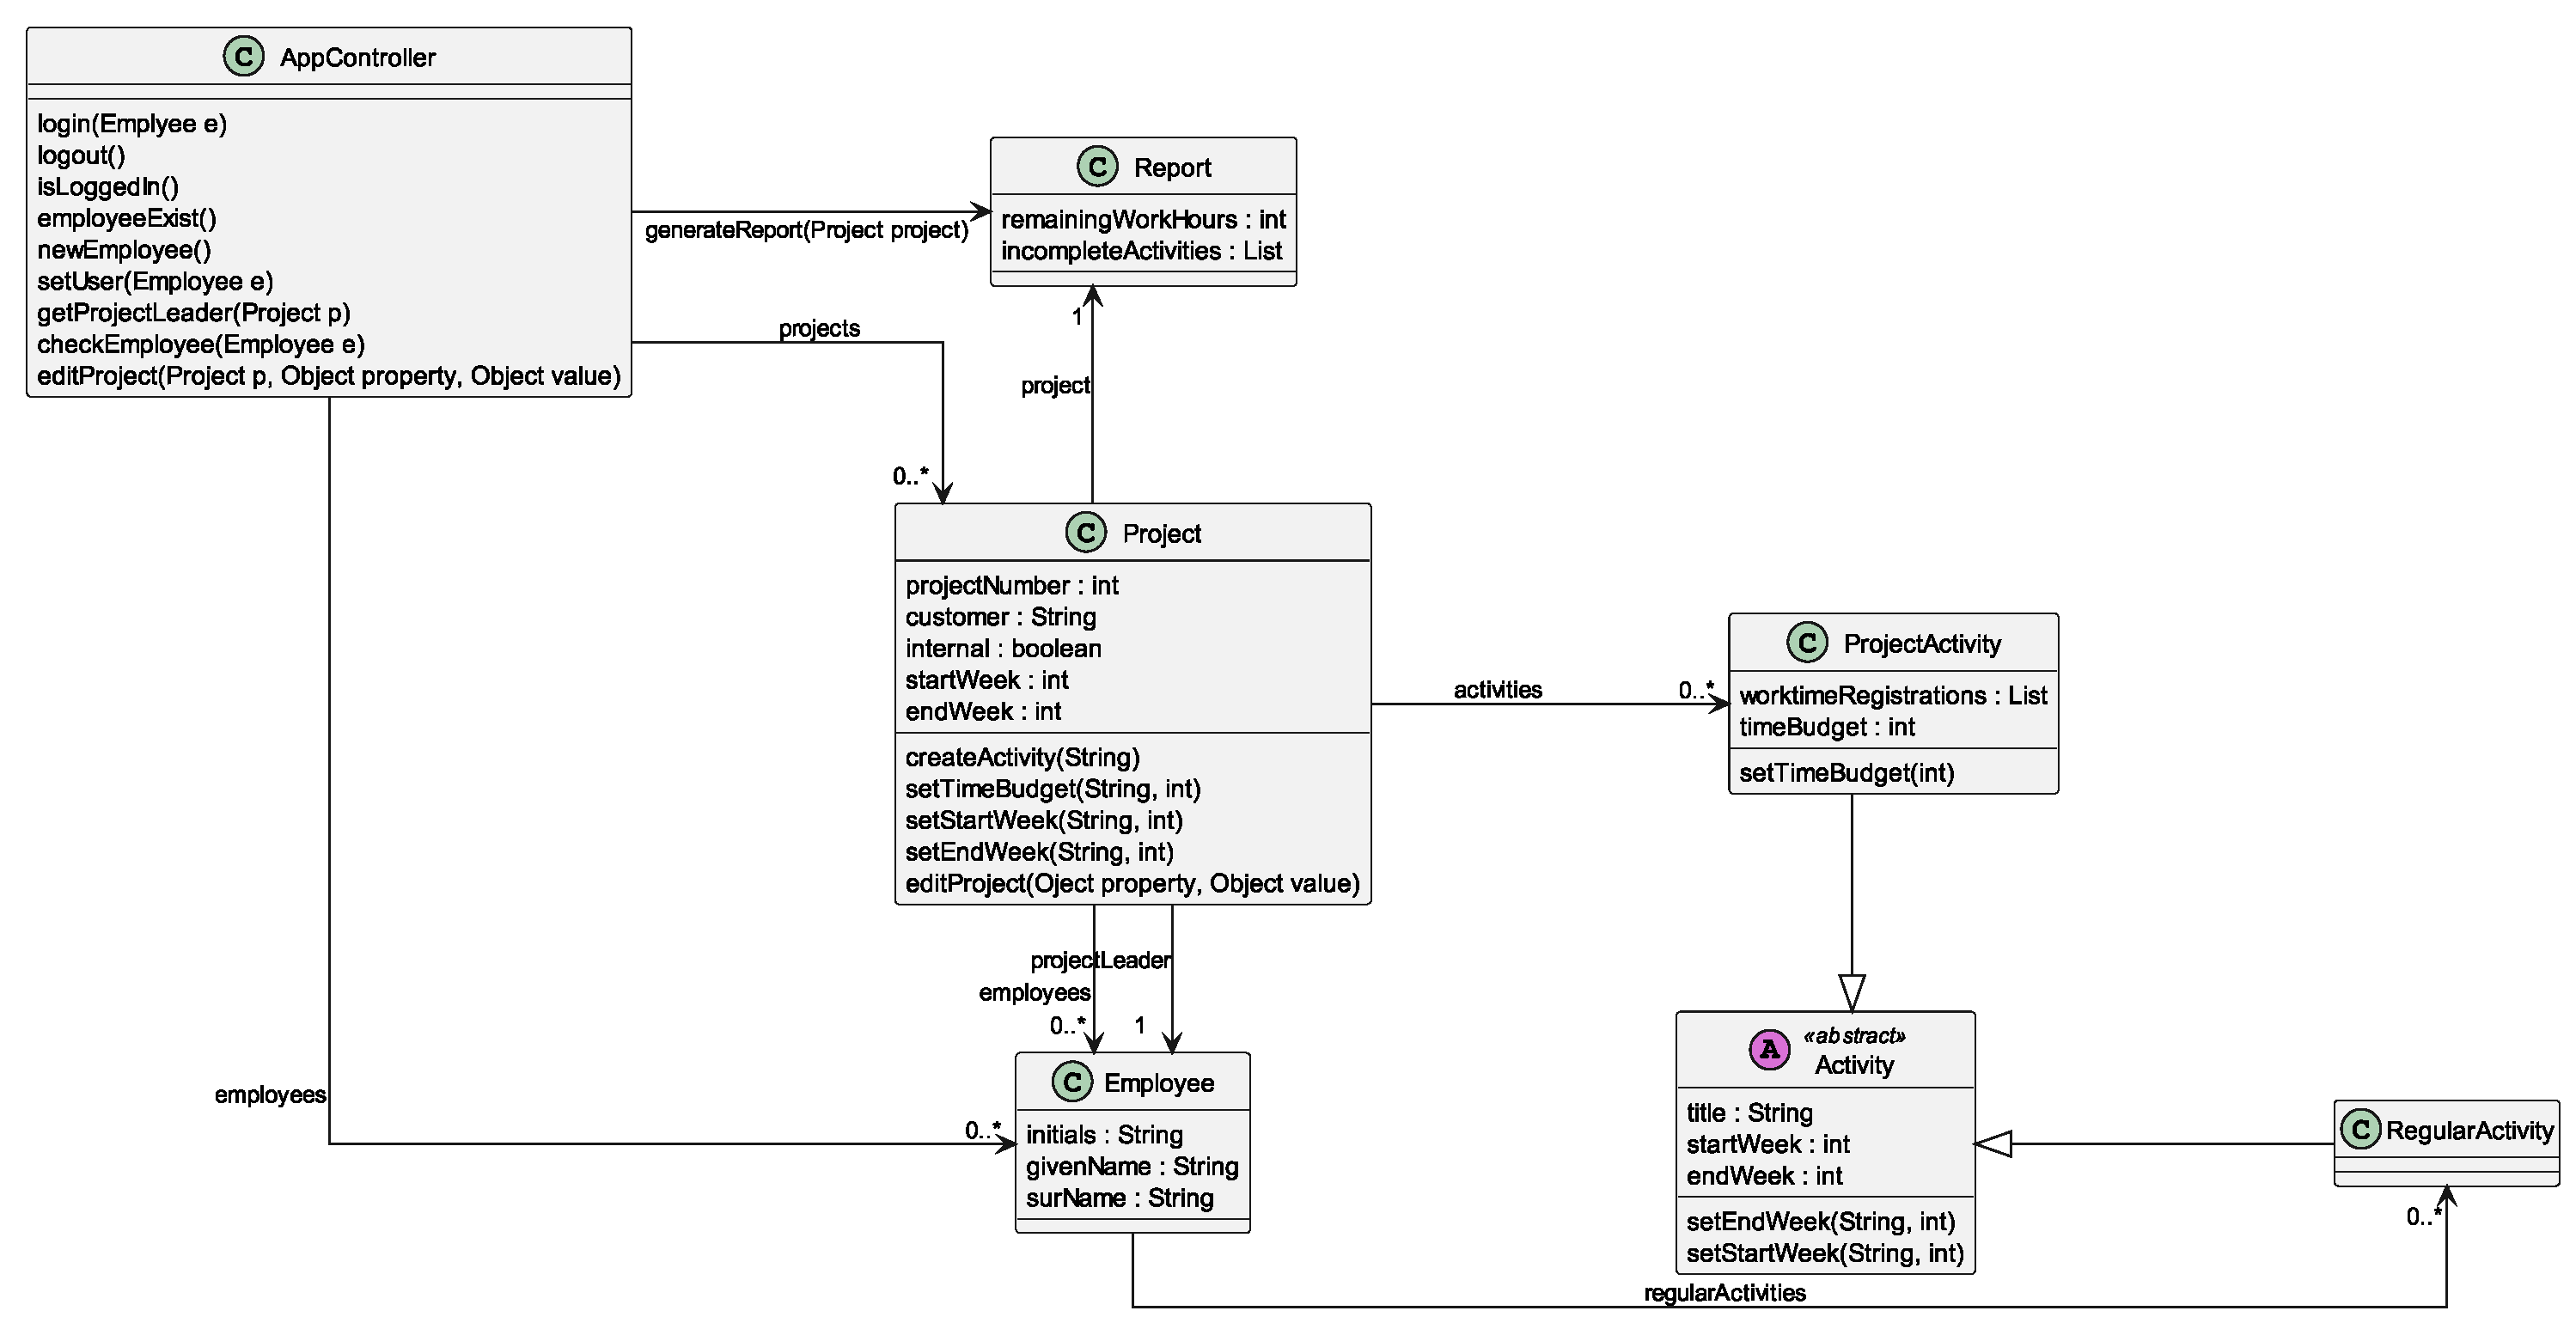
\includegraphics[width = \textwidth]{Diagrams/ClassDiagram.eps}
\end{figure}
\subsection{Sekvensdiagrammer}\label{sec:sequence}
% \begin{figure}[H]
%     \centering
%     \caption{Sekvensdiagram: Opret medarbejder}\label{fig:sequence_register_employee1}
%     \includegraphics[width = .75\textwidth]{Diagrams/seq_register_employee.png}
% \end{figure}
% \begin{figure}[H]
%     \centering
%     \caption{Sekvensdiagram: Opret medarbejder (et andet forslag)}\label{fig:sequence_register_employee2}
%     \includegraphics[width = 1\textwidth]{Diagrams/Register Employee.png}
% \end{figure}
\begin{figure}[H]
    \centering
    \caption{Sekvensdiagram: Opret medarbejder}\label{fig:sequenceRegisterEmployee}
    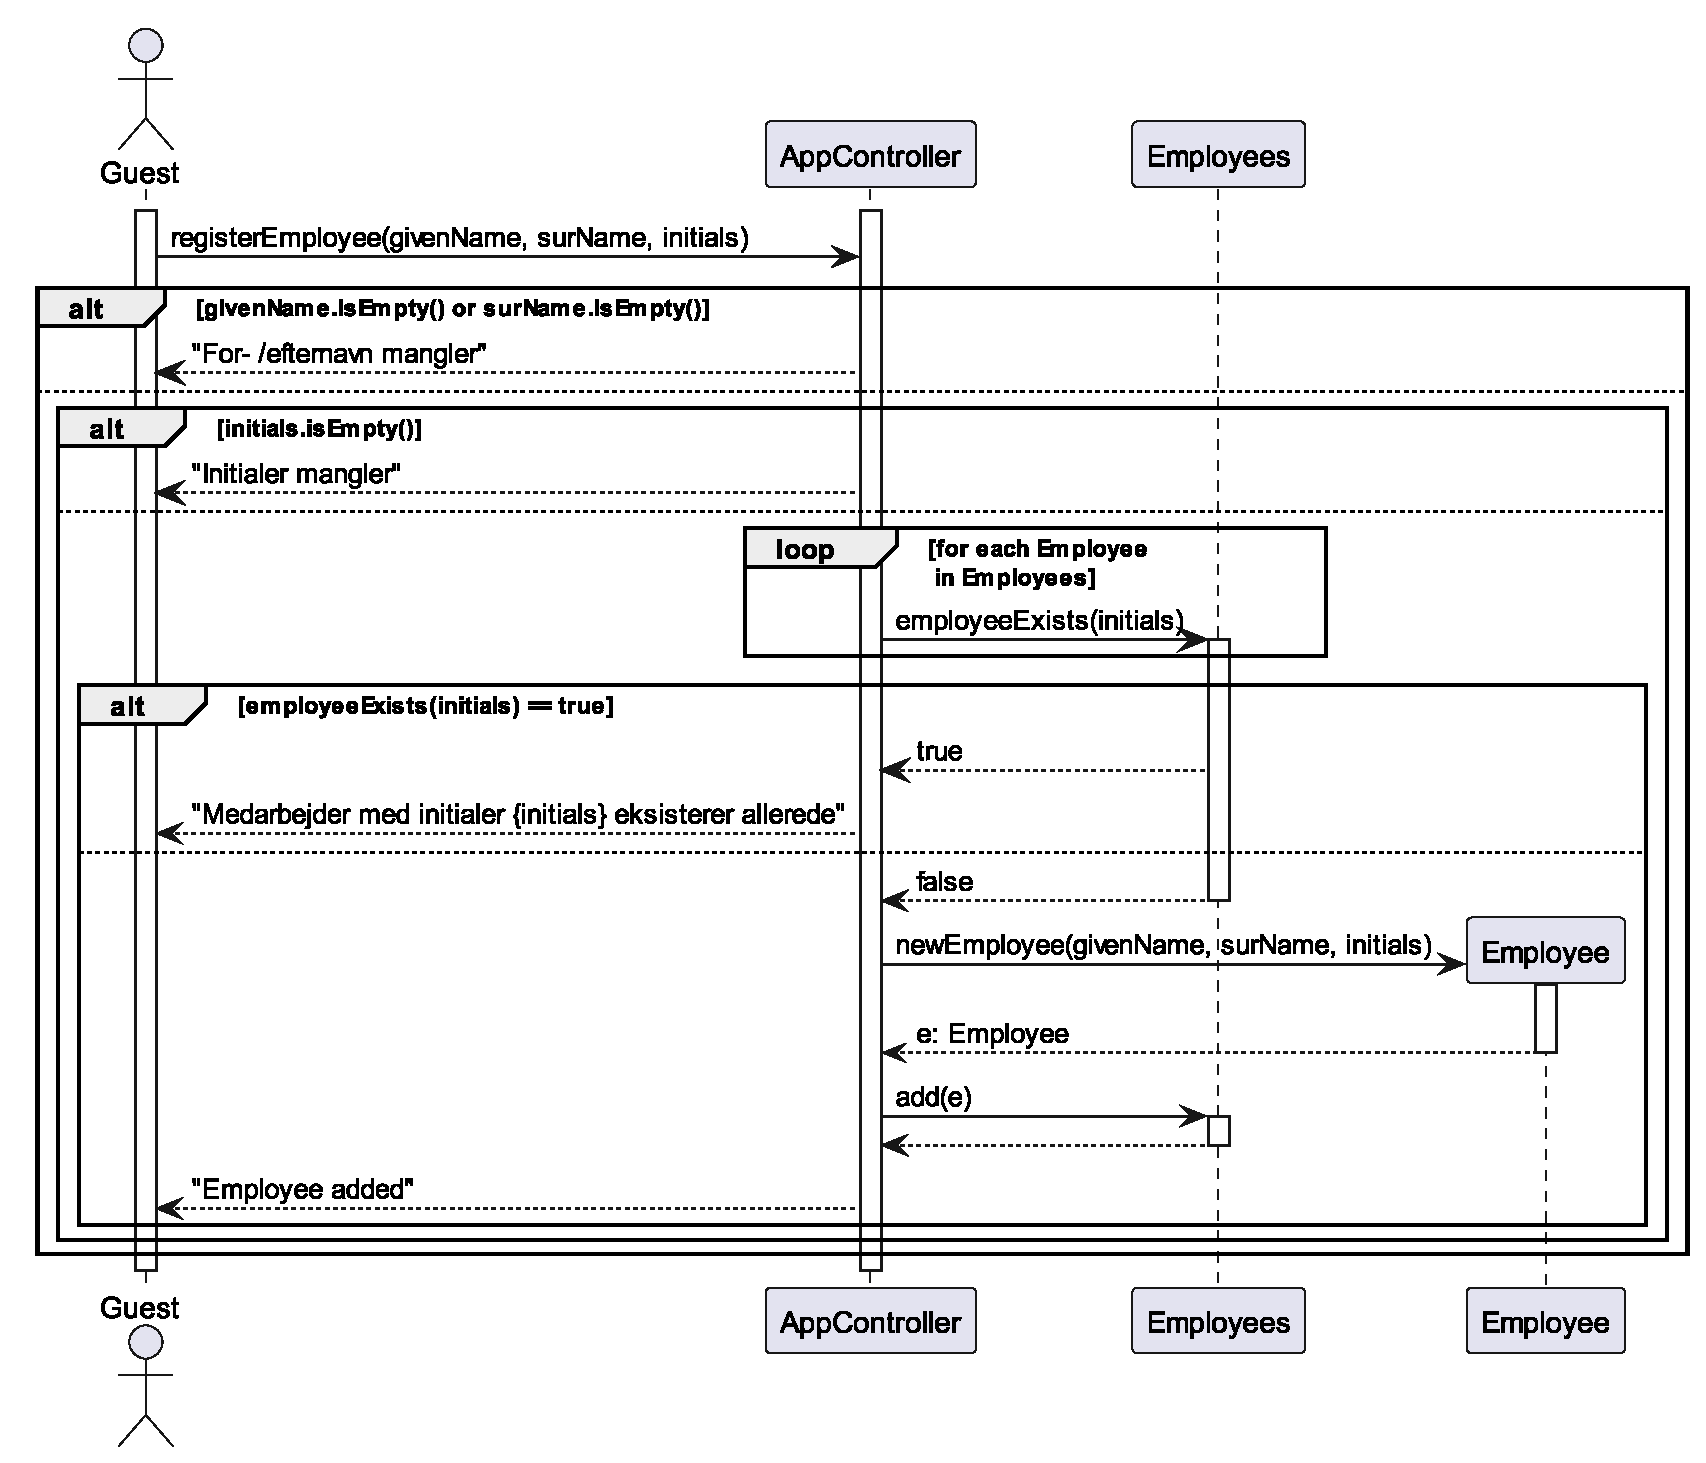
\includegraphics[width = .75\textwidth]{Diagrams/seq_registerEmployee.eps}
\end{figure}
\begin{figure}[H]
    \centering
    \caption{Sekvensdiagram: Medarbejder login}\label{fig:sequence_login}
    \includegraphics[width = .45\textwidth]{Diagrams/seq_login.png}
\end{figure}
\begin{figure}[H]
    \centering
    \caption{Sekvensdiagram: Medarbejder log ud}\label{fig:sequence_logout}
    \includegraphics[width = .25\textwidth]{Diagrams/seq_logout.png}
\end{figure}
\begin{figure}[H]
    \centering
    \caption{Sekvensdiagram: Opret projekt}\label{fig:sequence_create_project}
    \includegraphics[width = .75\textwidth]{Diagrams/seq_create_project.png}
\end{figure}
\begin{figure}[H]
    \centering
    \caption{Sekvensdiagram: Rediger projekt}\label{fig:sequence_project_edit}
    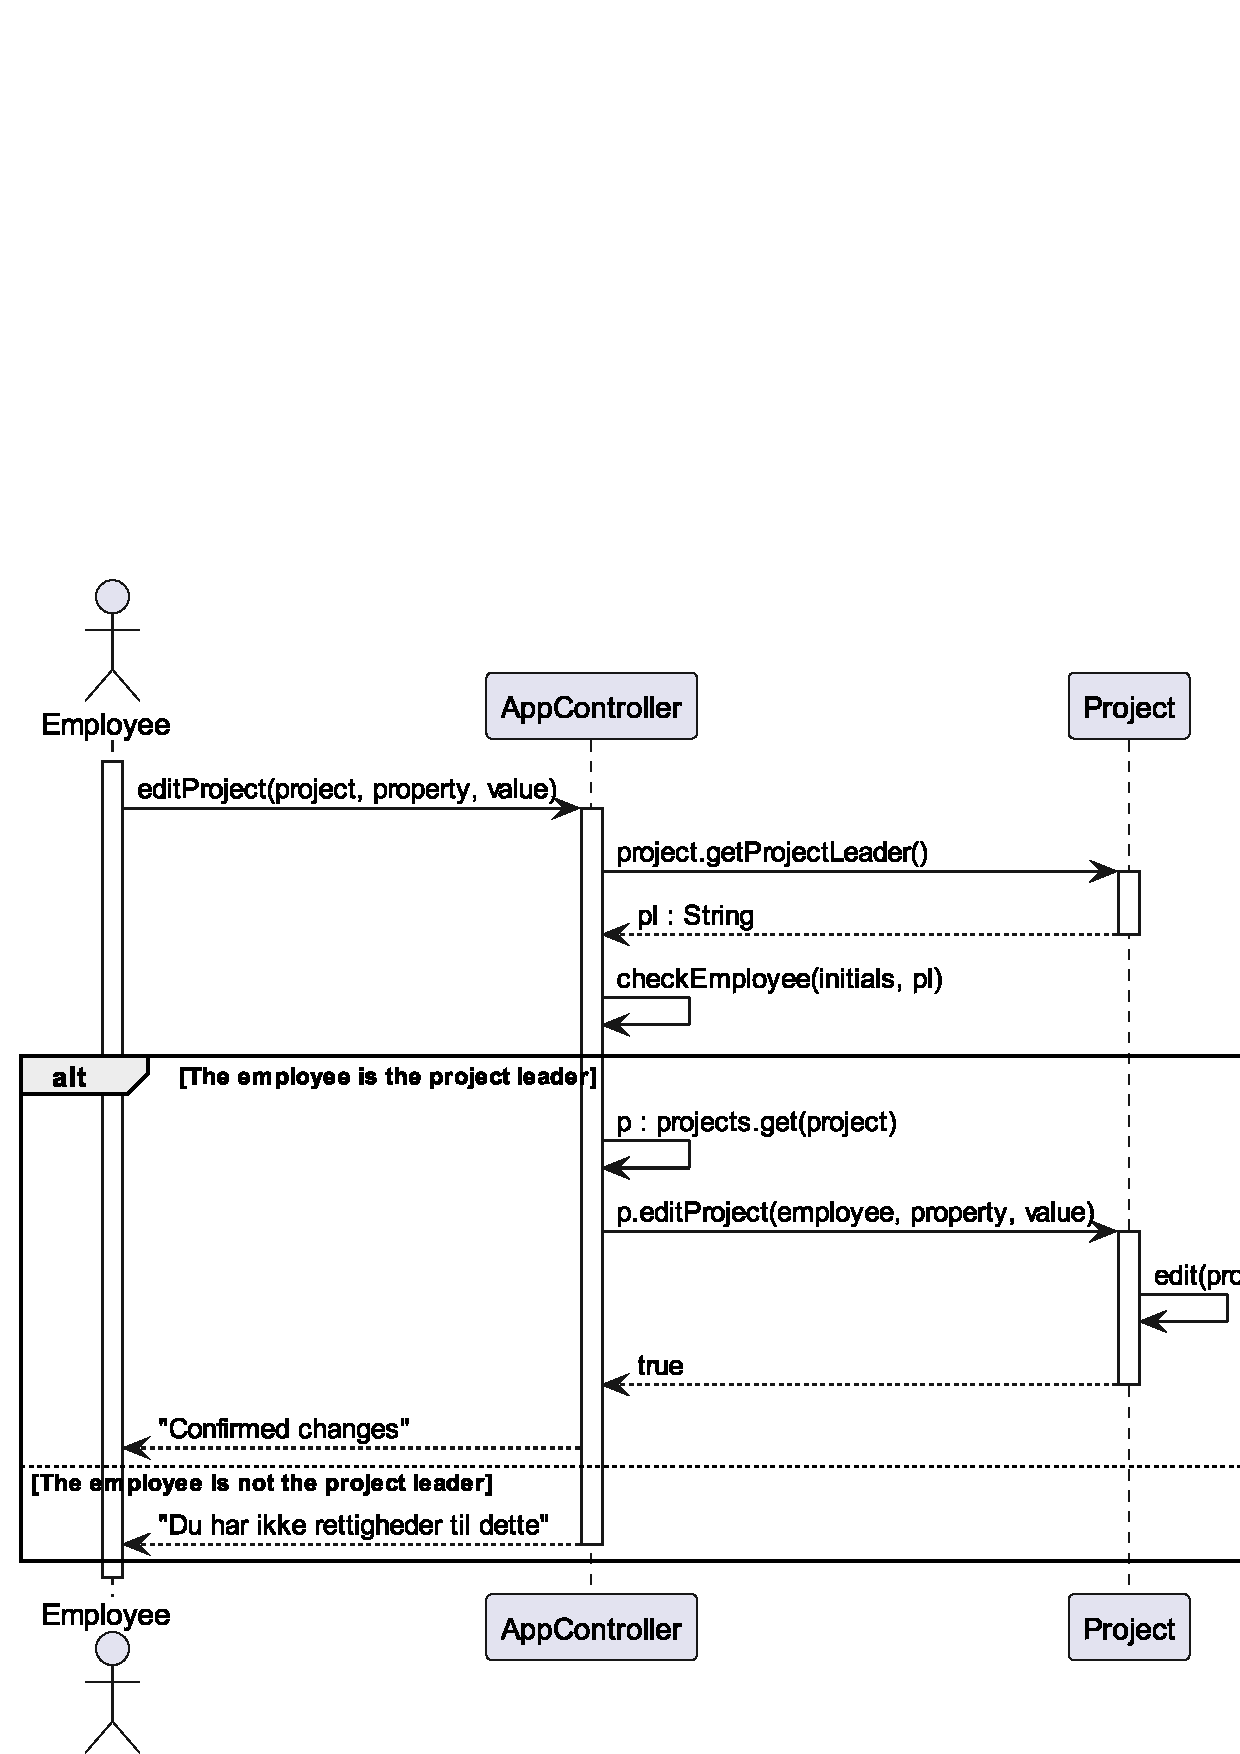
\includegraphics[width = .75\textwidth]{Diagrams/seq_project_edit.png}
\end{figure}
\begin{figure}[H]
    \centering
    \caption{Sekvensdiagram: Medarbejder udpeger sig som projektleder}\label{fig:becomeProjectLeader}
    \includegraphics[width = 1\textwidth]{Diagrams/Become Project Leader.png}
\end{figure}
\newpage
\section{Diskussion: Programdesign}
I dette afsnit bearbejdes to ting kort:
\begin{enumerate}
    \item Valg af datastrukturer
    \item Valg af klassestrukturer
\end{enumerate}
\subsection{Datastrukturer} I valg af datastrukturer er det vigtigt hvorledes vi henter og gemmer data. I programmet bliver medarbejdere og aktiviteter defineret med en unik streng, mens projekter bliver defineret med et løbenummer. Hvis man får nemheds skyld gemmer konvertere løbenummeret til en streng er der mulighed for at alle tre objekter kan gemmes i Map strukturer. Dette gør det nemt at hente objekter, udfører operationer på objekterne og overskrive objekterne i Map'et. Er det nødvendigt at iterere over et Map, kan man også nemt bruge Java's \mintinline{java}|.stream()| metode. Ønsker man at gemme brugt arbejdstid på en aktivitet er det derimod nemmest at gemme denne i en List, da arbejdstiden kun akkumuleres.
\subsection{Klassestrukturer} Programmet skal holdes simpelt og objekter skal nødvendigvis eje hinanden på en simpel måde. Det er besluttet at en \emph{Controller/Model}-klasse varetager programmets busniessstruktur. Hvis klassen bliver for kompliceret kan der senere indsættes en \emph{Viewer/Controller}-klasse som udelukkende varetager UI. Controller klassen indeholder Maps med projekter, medarbejdere og rapporter. Aktiviteter eksistere som en abstrakt klasse der nedarves til en fast aktivitet (f.eks. ferie), og projekt aktiviteter. De faster kan så ejes af et medarbejder objekt. Projektaktiviteter ejes af projekt objekter. Dermed bliver aktivitetsobjekter så ens som muligt, men ejes af de objekter der skal bruge dem.\newline
Til sidst findes \emph{worktimeRegistration}-klassen som varetager registrering af arbejdstid. Objektet ejes af en projektaktivitet, men henviser til medarbejder-objektet der udfører arbejdet. Således kan flere medarbejdere registrere arbejdstid på samme aktivitet.